% !TeX program = xelatex

\documentclass[12pt, a4paper]{article}

% Packages
\usepackage[inner=3.0cm, outer=3cm, top=2.5cm, bottom=2.5cm, includeheadfoot]{geometry}
\usepackage{graphicx}
\usepackage[spanish]{babel}
\usepackage{fancyhdr}
\usepackage{float}
\usepackage{setspace}
\usepackage{titlesec}
\usepackage[dvipsnames]{xcolor}
\usepackage[hidelinks]{hyperref}
\usepackage[utf8]{inputenc}
\usepackage{csquotes}  % Recomendado para biblatex
\usepackage[backend=biber,bibencoding=utf8,sorting=none]{biblatex} % Para bibliografía
\usepackage{listings}
%\usepackage{xcolor} % Para usar colores personalizados
\usepackage{caption}      % Para manejar captions
\usepackage{subcaption}   % Para las subfiguras
\usepackage{amsmath}
\usepackage{amssymb} 
\usepackage{comment}
\usepackage{appendix}
\usepackage{pdfpages}  % Paquete para insertar PDFs
\usepackage{xcolor} % Paquete básico para colorear tablas
\usepackage{array} % Para ajustar alineación de las columnas
\usepackage{cancel} % para cancelar valores en las ecuaciones


% Añadir archivo de bibliografía
\addbibresource{references.bib}

% Cambia el nombre del apéndice a "Apéndices"
\renewcommand{\appendixname}{Apéndices}
\renewcommand{\appendixtocname}{Apéndices}  % Cambia en el índice
\renewcommand{\appendixpagename}{Apéndices}  % Cambia en la página de título del apéndice
\renewcommand{\tablename}{Tabla}
\captionsetup[table]{name=Tabla} % Cambiar "Cuadro" por "Tabla"

% Header and Footer
\pagestyle{fancy}
\fancyhf{}
\fancyhead[L]{Generación de alta tensión}
\fancyfoot[L]{José Giménez Llanos - Álvaro Navarro Jorquera}
\fancyfoot[R]{\thepage}
\renewcommand{\footrulewidth}{0.4pt}
\setlength{\headheight}{14.5pt}

% Configuracion texto de código:
\lstset{
    language = Matlab,
  basicstyle=\ttfamily\footnotesize, % Si se quiere bastante mas pequeño sustituir \footnotesize por \scriptsize
  showspaces=false,           % No mostrar espacios con el símbolo ␣
  showstringspaces=false,     % No mostrar espacios en cadenas
  commentstyle=\color{green!60!black},
  keywordstyle=\color{blue},
  %stringstyle=\color{red},    % Color para las cadenas
  numberstyle=\tiny\color{blue},
  numbers=left,
  breaklines=true,
  frame=single,
  backgroundcolor=\color{gray!10},
  captionpos=b,
  caption=\lstname
}

\allowdisplaybreaks % Permite dividir alineaciones entre páginas

\begin{comment}



% Title Formatting
\titleformat{\section}{\normalfont\Large\bfseries}{\thesection}{1em}{}

% Cover Page
\title{
    \vspace{1cm} % Adjust vertical space
    %\includegraphics[width=0.55\textwidth]{MPOWER.jpg} \\ % Add your logo here (change "logo.png" to the actual filename)
    \begin{center}
        \begin{minipage}{0.3\textwidth}
            \includegraphics[width=\linewidth]{img/MPOWER.jpg} \\ % Logo 1
        \end{minipage}
        \hfill
        \begin{minipage}{0.3\textwidth}
            \includegraphics[width=\linewidth]{img/logo2.jpg} \\ % Logo 2
        \end{minipage}
        \hfill
        \begin{minipage}{0.3\textwidth}
            \includegraphics[width=\linewidth]{img/logo3.png} \\ % Logo 3
        \end{minipage}
    \end{center}
    \vspace{1cm} % Adjust vertical space after the logo
    \textbf{\Huge Diseño de una instalación fotovoltaica de utility scale} \\
    \vspace{1cm} % Adjust vertical space
    \large Energía Solar e Industria \\
    %\vspace{0.5cm} % Adjust vertical space
    %\large Date of Submission
}
\author{José Giménez Llanos}
\date{25/09/2024}
\end{comment}
\begin{document}

% Title Page
%\maketitle
\begin{titlepage}
    
    \newgeometry{ignoreall,top=2.5cm,bottom=1cm,outer=2.5cm,inner=2.5cm}
    \thispagestyle{empty}
    
    
\includepdf[pages=-]{portada2.pdf}
    
\end{titlepage}
    
% A partir de aquí aplica los márgenes establecidos en configuracioninicial.tex
\restoregeometry
\thispagestyle{empty}
\newpage

% Table of Contents
\setcounter{page}{1}

\tableofcontents

\listoffigures
\newpage

\setlength{\parskip}{6mm}


\section{Desarrollo de la propuesta}

Como ya se ha mencionado vamos a diseñar un circuito basado en multiplicadores 
de tensión o duplicadores de Greinacher para conseguir a la salida los $3kV$ 
especificados. 

En primer lugar, vamos a calcular cuántas celdas duplicadoras son necesarias 
en el diseño para obtener los $3kV$ a la salida. Para ello hay que tener en cuenta que el condensador 
de salida de
cada celda duplicadora se carga a una tensión igual al doble de la tensión de pico de la fuente, por lo que 
al poner varias celdas en serie, la tensión entre el terminal positivo del último condensador 
y la referencia (terminal negativo de la fuente) se irá duplicando. Por tanto, el cálculo 
queda de la siguiente manera:
\begin{equation}
    \text{nº duplicadores} = \frac{3000\,V}{220\cdot\sqrt{2}\cdot2} = 4.821 \approx 5
\end{equation}

Por tanto, con cinco duplicadores de tensión podemos obtener los $3kV$ de continua a partir 
de la fuente de $220 V_{rms}$. 
\begin{figure}[H]
    \centering
    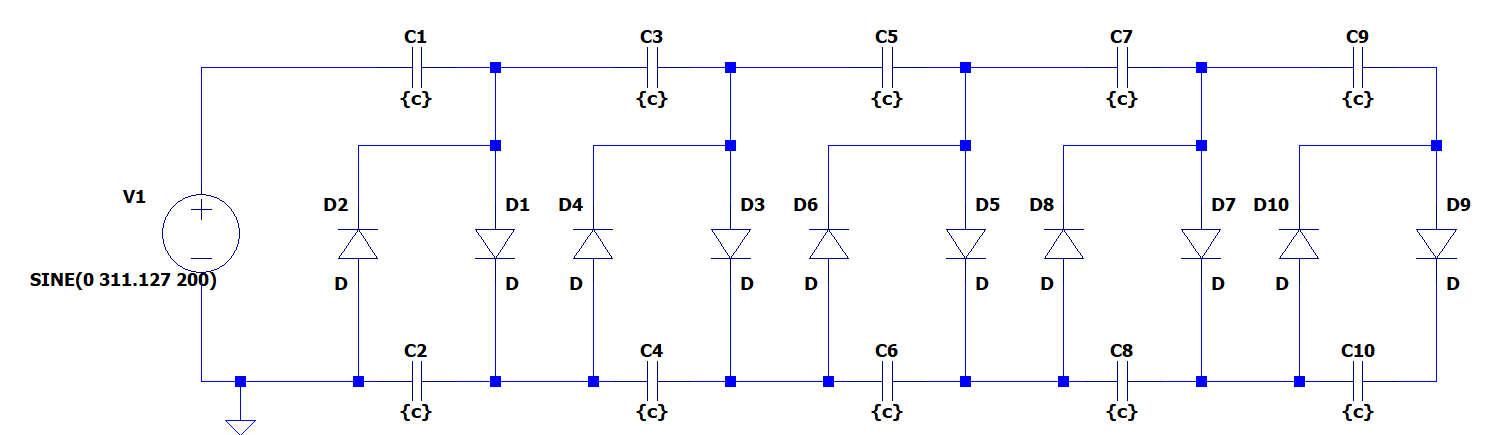
\includegraphics[width=0.9\textwidth]{img/mult_final.png}
    \caption{Esquema con los multiplicadores necesarios}
    \label{fig:esquema_mult}
\end{figure}

Con este esquema, idealmente y sin carga tendremos a la salida la siguiente tensión:
\begin{equation}
    V = 5\cdot2\cdot220\cdot\sqrt{2} = 3111.27\,V
\end{equation}

Por otro lado, la corriente de salida del circuito multiplicador tiene que se 
aproximadamente de $5 mA$. Para conseguir esta corriente de salida tenemos que calcular 
una carga que se conecte a la salida del multiplicador y que consuma esa corriente, ya que el multiplicador 
aislado, una vez se han cargado todos los condensadores, no consume ninguna corriente. La carga 
se puede calcular fácilmente mediante la Ley de Ohm:
\begin{equation}
    V = R\cdot I \rightarrow R = \frac{V}{I} = \frac{5\cdot2\cdot220\cdot\sqrt{2}}{0.005} = 622254\,\Omega
\end{equation}

Este consumo de corriente provoca que los condensadores se descarguen más rápidamente, aumentando 
el rizado y provocando una caída de tensión final, por lo que hay que emplear unos condensadores con 
una capacidad lo suficientemente elevada para minimizar el rizado y la caída de tensión. Además, esto producirá que el consumo de corriente
de la carga no sea exactamente igual al calculado, pero se asumirá este error puesto que el rizado y la caída de tensión son dependientes de la frecuencia
y el circuito debe ser capaz de funcionar en un rango de $50Hz$ a $200Hz$.

Como se ha mencionado en las especificaciones, el rizado máximo debe ser de un $\pm20\%$. En este caso 
realizaremos el diseño para tener un rizado de pico a pico de aproximadamente $10V$, que sería un 
rizado de aproximadamente $\pm8\%$. Para la obtención del rizado vamos a comenzar calculándolo 
en el supuesto de que solo tuviésemos una celda duplicadora. Si llamamos $t_1$ al tiempo en el que conduce el diodo que carga 
el condensador en cada ciclo y $t_2$ al tiempo en el que no conduce el diodo, es decir, el tiempo de descarga 
del condensador en cada ciclo, podemos expresar la corriente que el condensador aporta a la carga $R$ de la siguiente forma (llamamos 
q a la carga transferida en cada ciclo):
\begin{equation}
    I = \frac{dq}{dt} \approx \frac{q}{t_2}
\end{equation}

Como pasado el transitorio el tiempo $t_1$ es mucho menor que $t_2$ podemos aproximar 
$t_2$ de la siguiente forma:
\begin{equation}
    t_2 \approx \frac{1}{f}
\end{equation}

Por otro lado, sabemos que el rizado de tensión en un condensador en función de la carga transferida 
en un ciclo es el siguiente:
\begin{equation}
    \delta V = \frac{q}{C_2}
\end{equation}

Por tanto, combinando las tres ecuaciones anteriores obtenemos la siguiente ecuación:
\begin{equation}
    \delta V = \frac{I}{f\cdot C_2}
\end{equation}

No obstante, en una celda duplicadora, la carga primero se transfiere del condensador $C_1$ al condensador 
$C_2$, por lo que el rizado de pico a pico total a la salida de una sola celda duplicadora será el siguiente:
\begin{equation}
    \delta V = \frac{I}{fC_1}+\frac{2I}{fC_2} = \frac{I}{f}\left[\frac{1}{C_1}+\frac{1}{C_2}\right]
\end{equation}

Extrapolando este resultado a nuestro ejercicio y considerando todos los condensadores iguales con 
una capacidad $C$, el rizado de pico a pico queda de la siguiente forma:
\begin{equation}
    \delta V = \frac{I}{fC}[1+2+3+4+5]=\frac{I}{fC}\cdot15
\end{equation}

Por tanto, para obtener un rizado pico a pico de $10V$, la capacidad de los condensadores debe 
ser la siguiente:
\begin{equation}
    C = \frac{I}{\delta V\cdot f}\cdot15 = \frac{0.005}{10\cdot 50}\cdot 15 = 150\,\mu F
\end{equation}

El cálculo anterior se ha realizado para una frecuencia de $50Hz$ porque es más restrictivo, 
ya que a menor frecuencia mayor rizado. Podemos comprobar el rizado de pico a pico que se obtendrá con ese condensador 
a $200Hz$:
\begin{equation}
    \delta V = \frac{I}{fC}\cdot15 = \frac{0.005}{200\cdot 150\,\mu F}\cdot15 = 2.5\,V
\end{equation}

Por otro lado, podemos calcular la caída de tensión que va a provocar una carga con ese 
consumo de corriente. A partir de la expresión obtenida en la referencia \cite{park2015reduction}:
\begin{equation}
    V_{\text{drop}} = \frac{I}{fC}\left(\frac{2n^3}{3}+\frac{n^2}{2}-\frac{n}{6}\right)
\end{equation}

En la ecuación anterior, $n$ es el número de celdas duplicadoras, por lo que sustituyendo los datos a $50Hz$
la caída del voltaje final es la siguiente:
\begin{equation}
    V_{\text{drop}} = \frac{0.005}{50\cdot 150\,\mu F}\left(\frac{2\cdot5^3}{3}+\frac{5^2}{2}-\frac{5}{6}\right) = 63.33\,V
\end{equation}

Por tanto, el voltaje medio de salida que obtendremos con esa carga a $50Hz$ será el siguiente:
\begin{equation}
    V = 5\cdot2\cdot220\cdot\sqrt{2}-V_{\text{drop}} = 3047.93\,V
\end{equation}

Por otro lado, a $200Hz$ la tensión final será la siguiente:
\begin{equation}
    V_{\text{drop}} = \frac{0.005}{200\cdot 150\,\mu F}\left(\frac{2\cdot5^3}{3}+\frac{5^2}{2}-\frac{5}{6}\right) = 15.83\,V
\end{equation}
\begin{equation}
    V = 5\cdot2\cdot220\cdot\sqrt{2}-15.83= 3095.44\,V
\end{equation}

Por último, nos faltaría el diseño del circuito de medida. Este circuito de medida estará basado en 
un divisor de tensión para poder medir con un fondo de escala de $200V$. Además, la resistencia 
del multímetro es de $10M\Omega$. 

El circuito de medida para el que se van a realizar los cálculos es, por tanto, el siguiente:
\begin{figure}[H]
    \centering
    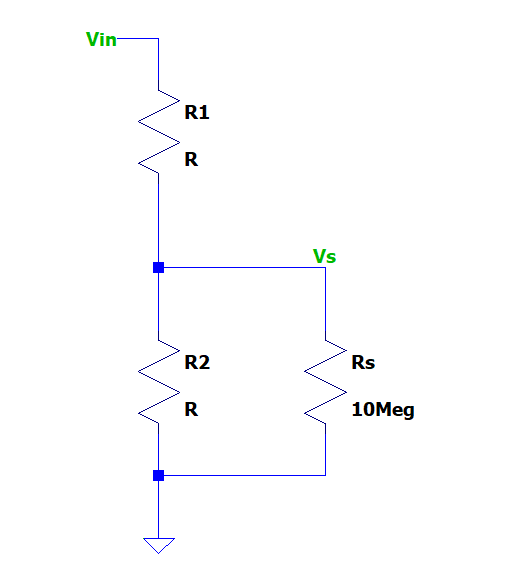
\includegraphics[width=0.4\textwidth]{img/circ_medida.png}
    \caption{Esquema para los cálculos del circuito de medida}
    \label{fig:esquema_med}
\end{figure}

Como valor de $V_{in}$ se selecciona la máxima tensión de salida que el circuito será capaz de proveer y 
dicha tensión se asociará con una caída en $R_2$ y $R_s$ de $200V$. De esta manera, nunca será posible sobrepasar
el fondo de escala. Dicho valor de $V_{in}$ es el siguiente:
\begin{equation}
    V_{in} = 5\cdot2\cdot\sqrt{2}\cdot220 = 3111.27\,V
\end{equation}

Por otro lado, queremos que $V_s$ sea igual a $200V$. Además, $R_2$ en paralelo con $R_s$ debe 
ser menor a 10 $M\Omega$. Si fijamos el valor del paralelo en 9 $\,M\Omega$ (valor elevado para minimizar el consumo del circuito) podemos calcular 
el valor de $R_2$:
\begin{equation}
    \frac{1}{9\,M\Omega} = \frac{1}{10\,M\Omega} +\frac{1}{R_2\,M\Omega} \rightarrow R_2 = 90\,M\Omega
\end{equation}

Por último, obtenemos el valor de $R_1$ a partir del divisor de tensión:
\begin{equation}
    V_s = Vin\cdot\frac{R_2//R_s}{R_1+R_2//R_s} \rightarrow R_1 = \frac{(R_2//R_s)\cdot(V_{in}-V_s)}{V_s}
\end{equation}

Sustituyendo valores, el valor de la resistencia $R_1$ queda:
\begin{equation}
    R_1 = \frac{9\,M\Omega\cdot(3111.27\,V-200\,V)}{200\,V} = 131.007\,M\Omega
\end{equation}

No obstante, uno de los requerimientos de diseño es que los componentes tuviesen una tensión de trabajo 
inferior a $1000V$. En la resistencia $R_1$ en las condiciones de diseño va a caer aproximadamente la siguiente tensión:
\begin{equation}
    V_{R1} = 3111.27\,V-200\,V = 2911.27\,V > 1000\,V
\end{equation}

Por tanto, si dividimos la resistencia $R_1$ en tres resistencias iguales, cada una tendrá una 
tensión de trabajo igual a un tercio de la tensión de trabajo de $R_1$, es decir:
\begin{equation}
    V_{R'} = \frac{V_{R1}}{3} = \frac{2911.27}{3} = 970.42\,V < 1000\,V
\end{equation}

Por tanto, el circuito final del multiplicador de tensión con la carga y el circuito de medida 
de tensión queda de la siguiente manera:
\begin{figure}[H]
    \centering
    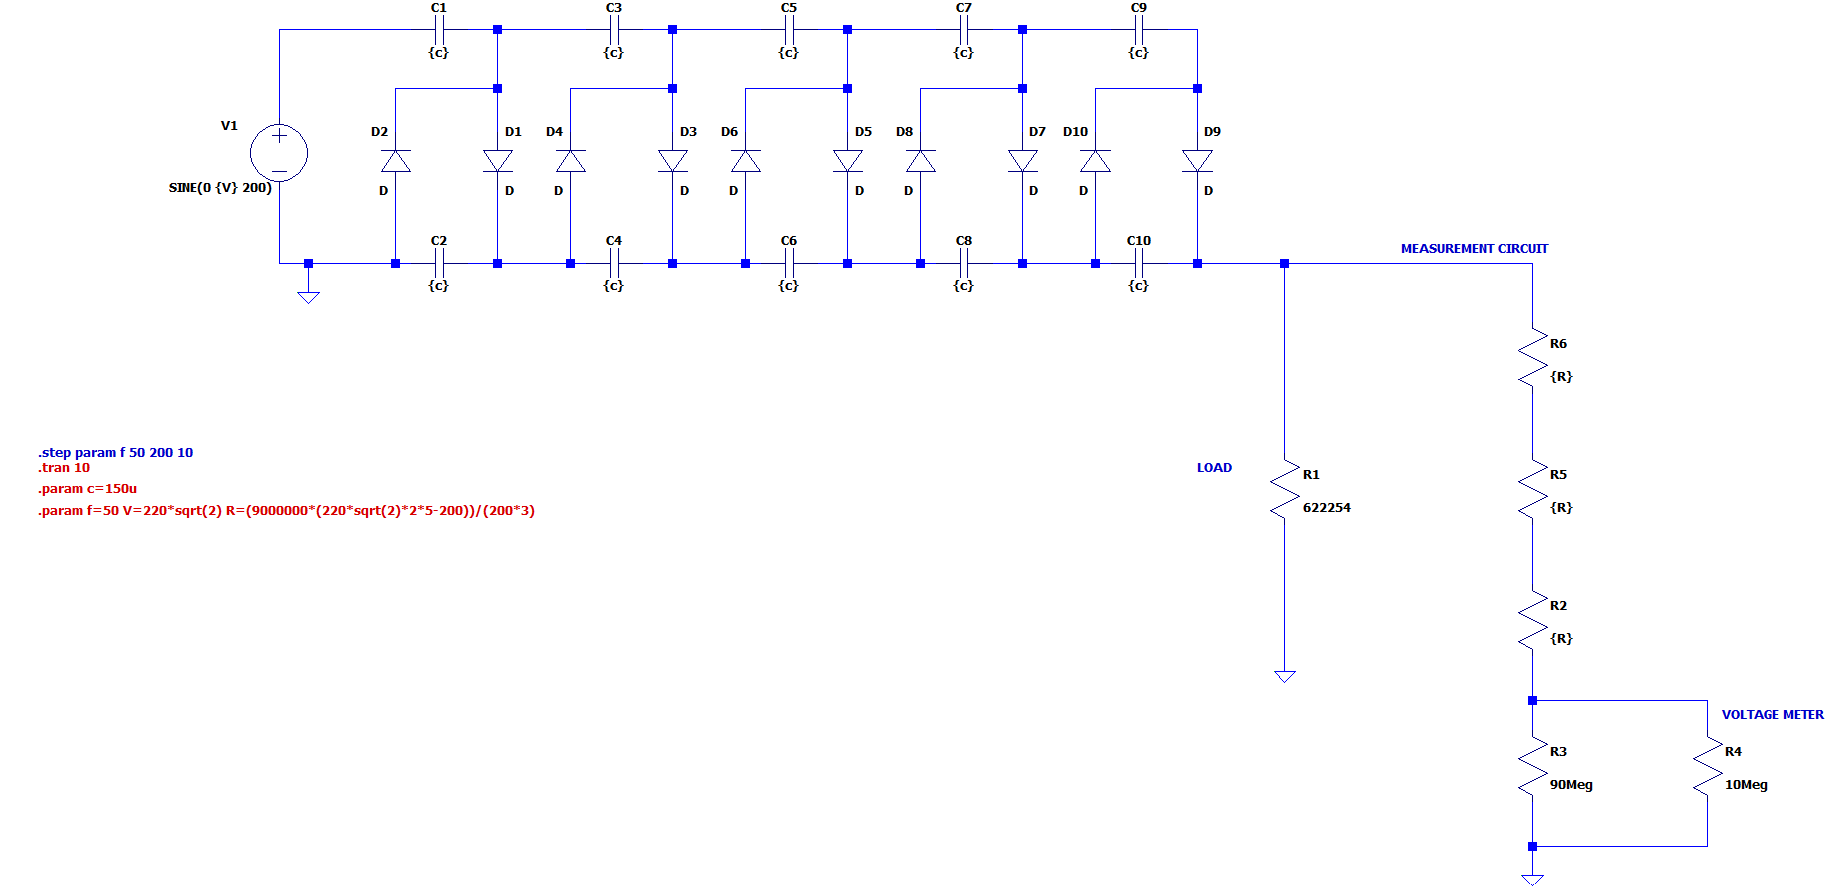
\includegraphics[width=1\textwidth]{img/circ_final.png}
    \caption{Circuito multiplicador de tensión diseñado}
    \label{fig:esquema_final}
\end{figure}

Por último, podemos calcular el consumo de corriente máxima aproximado del circuito de medida\footnote{Nos referimos 
a la corriente máxima que consume el circuito de medida, porque estamos considerando la tensión 
de salida teórica sin caída debido a la carga.}:
\begin{equation}
    I_{meas} = \frac{V_{in}}{R_{total}} = \frac{3111.27}{9\,M\Omega+131.007\,M\Omega} = 22.22\,\mu A
\end{equation}
\section{Introducción}

En este entregable se realiza el diseño y análisis de un circuito multiplicador de tensión basado en el Duplicador de Greinacher.
Este circuito, el cual se puede ver en la figura \ref{fig_intro}, se basa en el principio del rectificador de medio puente.

El condensador $C1$ se carga para tensiones de entrada desde $-\hat{V}$ hasta $+\hat{V}$ ($\frac{dV}{dt}$ positivo) y
se descarga a través del diodo $D2$ durante las variaciones de tensión de entrada $\frac{dV}{dt}$ negativas, cargando así el condensador
$C2$. Este proceso se repite durante varios ciclos, hasta llegar a un punto en el que el condensador $C1$ quede cargado a la tensión de pico de la 
senoidal de entrada y el condensador $C2$ al doble de la tensión de pico de entrada. Esto se produce puesto que,
en los ciclos de tensión de entrada negativa, la tensión soportada por el condensador $C2$ es la del condensador $C1$ sumada a la tensión de la fuente.

\begin{figure}[H]
    \centering
    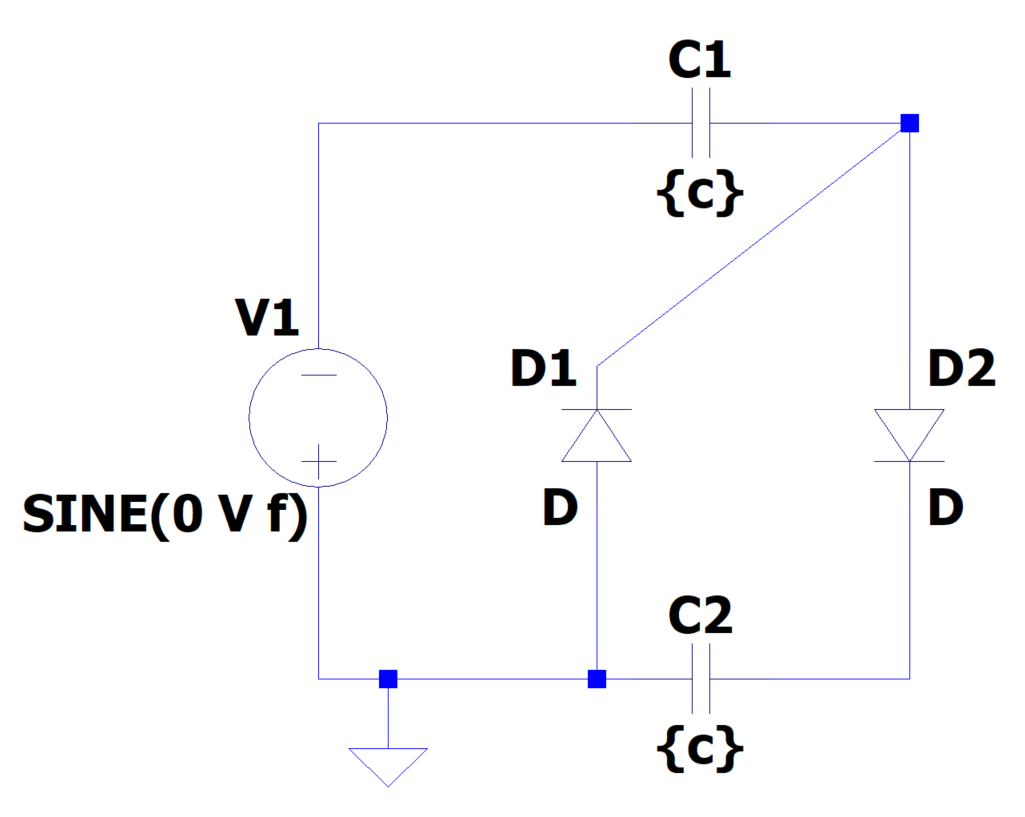
\includegraphics[width=0.6\textwidth]{Imagenes_alvaro/fig_intro.png}
    \caption{Multiplicador de Greinacher de 1 etapa}
    \label{fig_intro}
\end{figure}

Además, cabe destacar que este circuito es escalable, permitiendo de manera teórica obtener tensiones de salida infinitas a partir de fuentes de tensión
oscilatorias de bajo voltaje.

\section{Objetivos}

El principal objetivo de este trabajo es conseguir diseñar un Multiplicador de Greinacher que permita obtener una tensión de salida específica.
Además, debe ser capaz de proveer cierta cantidad de corriente de salida sin que se produzca una caída significativa de la tensión, de manera que será
necesario dimensionar correctamente la capacidad de los condensadores. Por otra parte, el circuito debe ser capaz de funcionar en un rango de frecuencia definido
y para tensiones de entrada senoidales y cuadradas. También será necesario diseñar un circuito que permita medir la tensión de salida a partir de un multímetro.
Todos los requisitos se definen de manera específica en la sección \ref{requisitos}.

\section{Estado de la técnica}

Para la construcción del Multiplicador de Greinacher será necesario obtener el número de etapas necesarias a partir de la tensión de pico de entrada y
la tensión continua requerida a la salida. A partir de ahí se seleccionarán los componentes (diodos y condensadores), los cuales deben ser capaces de soportar las tensiones máximas
a las que se puedan someter.

Respecto a la carga, puesto que la tensión de salida es continua, se dimensionará una resistencia para que circule a través de la misma la corriente deseada.
Dicha resistencia, en el circuito real, deberá ser seleccionada para que pueda soportar la potencia a disipar. Puesto que la tensión de salida será elevada,
corrientes de miliamperios pueden producir potencias de decenas de vatios que deberán ser disipadas por la resistencia.

Para el diseño del circuito de medida de tensión, se utilizará un divisor resistivo con un multímetro en paralelo con la resistencia de debajo del divisor.
De esta manera, la resistencia total de debajo del divisor estará limitada por la resistencia del multímetro. Consecuentemente, puesto
que se debe construir el circuito para obtener corrientes mínimas, se diseñará para que la resistencia de debajo del puente total sea lo más cercana posible a la
resistencia del multímetro.

\section{Establecimiento de requerimientos} \label{requisitos}

Los requerimientos del circuito se dividen, en este caso, en los requerimientos del Multiplicador de Greinacher y los del equipo de monitorización
de tensión de salida. Los requerimientos del Multiplicador de Greinacher son los siguientes:

\begin{itemize}
    \item Tensión de salida: $3kV \pm 5\%\,\, \left(DC\right)$
    \item Corriente de salida: $~5mA$
    \item Rizado máximo: $\pm 10\%$
    \item Tensión de entrada: $220V\,\, \left(AC\right)$
    \item Tensión de trabajo de componentes: $<1000V$
    \item Rango de frecuencia de entrada: $\left[50Hz, 200Hz\right]$
    \item Forma de tensión: senoidal o cuadrada
\end{itemize}

Respecto al equipo de monitorización, debe cumplir los siguientes requisitos para que el funcionamiento del circuito se vea 
lo menos afectado posible al utilizarlo:

\begin{itemize}
    \item Consumo de corriente mínimo
    \item Tensión máxima de $200V$, correspondiente con la tensión máxima de salida
\end{itemize}




\begin{comment}
    
% 4. Measurement/Testing Results
\section{Measurement}
Summarize the data gathered during the lab, including measurements and observations.
\begin{figure}[h!]
    \centering
    \includegraphics[width=0.8\textwidth]{example-image} % Example of adding a figure
    \caption{Test results for circuit 1}
    \label{fig:circuit1}
\end{figure}

% 5. Analysis and Discussion
\section{Analysis and Discussion}
Interpret the results obtained. Compare them with theoretical values, explain discrepancies, and discuss their significance.

% 6. Recommendations/Conclusions
\section{Conclusions}
Provide conclusions based on the results and discuss any recommendations for improvements, future work, or alternative solutions.
\end{comment}
%\newpage

%%%%%CUIDADO EN ESTE CASO ESPECIFICAMENTE HE QUERIDO PONER LAS REFERENCIAS DESPUES DE LOS ANEXOS PERO GENERALMENTE NO ES ASI
%\nocite{*} % Esto incluirá todas las referencias del archivo .bib
%\printbibliography[heading=bibintoc, title={Referencias}]

%\input{anexos}


% Bibliography
\newpage
\nocite{*} % Esto incluirá todas las referencias del archivo .bib
\printbibliography[heading=bibintoc, title={Referencias}]
\end{document}

